\documentclass[12pt,a4paper]{article}
\usepackage[T1]{fontenc}
\usepackage[utf8]{inputenc}
\usepackage{lmodern,microtype,amsmath,amssymb,graphicx,booktabs,array}
\usepackage[margin=25mm]{geometry}
\usepackage[authoryear,round]{natbib}
\usepackage[hidelinks]{hyperref}
\usepackage{fancyhdr}
\usepackage{setspace,lineno}
\doublespacing
\pagestyle{fancy}\fancyhf{}\fancyhead[L]{AMP evaluation: review candidate}\fancyhead[R]{12 October 2026}\fancyfoot[C]{\thepage}
\setlength{\headheight}{15pt}
\newcommand{\mmd}{\mathrm{MMD}^{2}}
\newcommand{\ug}{\ensuremath{\mu\mathrm{g}/\mathrm{mL}}}
\title{Reconstruction gains without superiority over an autoregressive comparator:\\a bounded antimicrobial peptide evaluation}
\author{Hongsheng Wang\textsuperscript{1}, Jie Yang\textsuperscript{2}, Feng Lin\textsuperscript{3}, Fei Wu\textsuperscript{1}\\[3pt]
\small \textsuperscript{1}Zhejiang University, Zhejiang, China\\
\small \textsuperscript{2}Hangzhou Dianzi University, Zhejiang, China\\
\small \textsuperscript{3}Fuyao University of Science and Technology, Fujian, China}
\date{Complete review candidate; author details and submission approval unconfirmed}
\begin{document}
\linenumbers
\maketitle
\noindent\textbf{Review status.} This candidate integrates completed computational development experiments and separately identified historical records. It is not cleared for journal submission. The named authors and affiliations are transcribed from the frozen v6-r3 manuscript, not newly verified. No new laboratory validation is reported.

\begin{abstract}
\noindent\textbf{Motivation:} Sequence reconstruction, generated-sequence similarity and measured antibacterial activity address different questions. A practical evaluation must distinguish improvements to one component from evidence for the complete design process.\\
\textbf{Results:} We evaluated a retrieved antimicrobial peptide pipeline using 279 training sequences and a repeatedly accessed 41-sequence development set. In a fixed, single-seed comparison, a 21-class cross-entropy reconstruction objective achieved 497/701 correctly reconstructed development residues (70.90\%), compared with 88/701 (12.55\%) for a same-capacity raw one-hot squared-error objective. Both used the same legal-prefix decoder. With matching diffusion training and 16 requests per terminal condition, cross-entropy also improved all six prespecified sequence-distribution distances relative to the squared-error pipeline. However, a terminal-conditioned LSTM had lower distances still, in both terminal conditions and against both reference sets. This does not establish a general superiority of the LSTM: tuning adequacy, independent confirmation and biological endpoints are absent. Subsequent latent-variable diagnostics and exploratory MIC prediction did not establish a successful repair. Historical records for 27 peptides are reported separately; missing assay semantics and generation provenance prevent their use as validation of these new runs.\\
\textbf{Availability and implementation:} The review package contains source-bound summaries, analysis code and supplementary tables. Complete public data and model release remains unresolved.\\
\textbf{Supplementary information:} Complete distance tables, execution details, negative follow-ups and historical records accompany this candidate.\\
\textbf{Contact:} Historical corresponding author: Jie Yang; \texttt{yangjie08@hdu.edu.cn} (unconfirmed).
\end{abstract}

\section{Introduction}
Antimicrobial peptide generation produces sequences for subsequent characterization. Reconstruction of a known sequence, resemblance to an observed sequence distribution, and antibacterial activity of a synthesized material are distinct outcomes. A model can improve reconstruction without generating better candidates from its sampling distribution. Similarly, matching residue frequencies or peptide lengths does not demonstrate a useful activity spectrum, low toxicity or acceptable stability.

Variational autoencoders (VAEs) learn latent representations by combining reconstruction and regularization objectives \citep{kingma2014}. Denoising diffusion models provide a separate mechanism for sampling a learned distribution \citep{ho2020}. Peptide design has also used recurrent sequence models \citep{muller2018} and conditional VAEs with downstream selection and experimental assessment \citep{szymczak2023}. These precedents make an autoregressive comparator and explicit separation of generation from selection necessary parts of an evaluation. They do not provide interchangeable numerical baselines: published data, selection and assays differ.

A recent comparative study already distinguishes autoencoder reconstruction from generation evaluation and examines multiple AMP model families \citep{beierle2026}. QMAP likewise provides an established benchmark for MIC and hemolytic-activity regression with explicit evaluation splits \citep{qmap2026}. We do not claim to introduce either evaluation principle. AMPGen further illustrates a diffusion-based design with downstream selection and linked assays \citep{ampgen2025}. Its biological evidence is not evidence for the experiments reported here.

The inspected AMP implementation uses a convolutional VAE with sequence-derived descriptors and a diffusion model over posterior parameters. Its historical records do not identify the configuration and checkpoint responsible for each reported peptide. We therefore distinguish a new, bounded computational development experiment from historical biological observations. The computational objective is to assess whether replacing a scalar or squared-error reconstruction path with categorical reconstruction improves both reconstruction and the complete sampling path under fixed operating conditions.

The contribution of this report is an implementation-specific evaluation, not a new learning algorithm or a representative benchmark. It contains a same-capacity loss comparison, a runnable terminal-conditioned autoregressive comparator, preserved unsuccessful follow-up diagnostics, and an explicit account of what the historical material can support. The main observation is that an improvement over the matched squared-error pipeline does not establish superiority over a separate autoregressive generator. The report also identifies the evidence missing for a broader claim. We do not infer that VAEs or diffusion models generally fail for AMP design.

\section{Materials and methods}
\subsection{Evidence sources and evaluation scope}
The inspected code snapshot is commit \nolinkurl{e7486fb714cbf5c663cc01052e42fb63d4ba3a40} of the AMP repository. Snapshot identity establishes the inspected implementation, not its use in a historical experiment. The frozen v6-r3 manuscript and earlier runs were preserved. All work reported here was performed in a separate development workspace.

The cohort was derived from a frozen, bounded collection of 512 official DBAASP detail cards. Eligibility required an unchanged canonical 1--48-residue monomer sequence, an unmodified N terminus, a free or amidated C terminus, compatible provider molecular graphs and traceable bacterial MIC metadata. Explicit sequence and chemistry exclusions were retained. The active chemistry gate required an exact provider match plus, for other providers, only independently checked neutral arginine/histidine local tautomer relations; it was not a general graph-normalization rule. This is a selected metadata-qualified cohort, not a set of independently confirmed active peptides.

Sequence grouping used global Needleman--Wunsch identity of at least 70\%, counting all alignment columns including gaps, and transitive connected components. Historical exposed components were assigned to training or excluded under the frozen exposure rules; previously unexposed components received a seeded hash assignment with nominal 80/10/10 proportions. The retained train/development files were released separately from the reserved partition. Descriptor scaling was fitted on training data only. Free and amidated sequences are not matched versions of the same sequence; terminal-group comparisons do not estimate a chemical-modification effect.

The main experiment used a fixed 279-sequence training partition and a 41-sequence development partition. Free and amidated terminal groups contained 126 and 153 training sequences, and 18 and 23 development sequences, respectively. The development set contains 701 non-padding residues. Neither an independent final evaluation nor a new laboratory experiment was performed. The reserved evaluation partition remained unopened. The development set had already informed previous investigation; it is not an untouched confirmation sample. Dataset and code hashes, configurations and execution rules were frozen before the corresponding natural runs, but this does not remove the prior exposure of the development data.

Terminal state is the only externally supplied condition during the main generation experiment. No true sequence, residue-aligned descriptor or true peptide length is supplied to the generator. Sequence-derived descriptors remain available to the encoder during reconstruction and training. Reconstruction therefore has substantially more input information than de novo generation. Historical activity-class labels are not treated as verified biological conditions in the new experiment.

\subsection{Reconstruction objectives and legal-prefix decoding}
The CE21 and MSE21 models share the same VAE architecture, initialization, batches, random-number schedule, 48-position output, 21-category head and decoding rule. The output categories are the 20 canonical amino acids and padding. Each model has 1,681,549 parameters, including 357 output-head parameters. Let $s_{ijc}$ denote the raw score for category $c$ at position $j$ in sample $i$, and let $y_{ij}$ include the padding target. For batch size $B$, the two reconstruction objectives are
\begin{align}
 L_{\mathrm{CE}}&=-\frac{1}{48B}\sum_{i,j}\log\operatorname{softmax}(s_{ij})_{y_{ij}},\\
 L_{\mathrm{MSE21}}&=\frac{1}{2(48B)}\sum_{i,j,c}\bigl(s_{ijc}-\mathbf{1}[c=y_{ij}]\bigr)^2.
\end{align}
Both add the retrieved flow-dependent KL density term normalized by $48B$, with coefficient one. The fixed coefficient does not equate the effective reconstruction-to-KL scale across losses. This comparison isolates the implemented loss form at a fixed coefficient; it is not an optimization over scale-matched objectives.

For either head, legal-prefix decoding chooses a length $l\in\{0,\ldots,48\}$ by maximizing
\begin{equation}
 J(l)=\sum_{j\leq l}\max_{c\ne\mathrm{PAD}}s_{jc}+\sum_{j>l}s_{j,\mathrm{PAD}}.
\end{equation}
Ties between lengths select the smallest maximizing length. It then selects the highest-scoring non-padding category in the prefix and padding in the suffix. Adding a position-specific softmax normalization changes all length scores by the same total, so raw-score and log-softmax formulations yield the same maximizer. This rule supplies no true length. It is a standard constrained readout and is not claimed as a novel algorithm.

The scalar comparator preserves the legacy integer-target squared-error path and round, clamp and first-padding readout. It has 1,681,209 parameters and a 17-parameter output head. Its target encoding, normalization, KL scaling and decoding differ from CE21; it is a complete legacy-pipeline comparator, not a single-factor ablation. Padding slots contribute to its reconstruction numerator, despite the non-padding denominator.

\subsection{Posterior-parameter diffusion and autoregressive comparator}
For each VAE, the encoder is frozen after training. Its posterior mean $\mu$ and log-standard deviation $\ell$ are stacked as the clean diffusion target $U_0$. A denoiser predicts the Gaussian noise added to that tensor. Reverse diffusion produces $\widehat\mu$ and $\widehat\ell$; a separate draw then forms
\begin{equation}
 z=\widehat\mu+\exp(\widehat\ell)\odot\epsilon,\qquad \epsilon\sim\mathcal N(0,I),
\end{equation}
which is passed directly to the matching decoder. No inverse prior-flow operation is applied to this posterior-coordinate latent. The diffusion model is retrained for each VAE representation; an old diffusion checkpoint is not relabeled as matching a newly trained encoder.

The autoregressive comparator has two LSTM layers with hidden width 64, token embeddings of width 32, terminal embeddings of width 8 and 62,501 parameters. It is trained with teacher-forced token prediction and generates from the terminal condition and its own sampled prefix. An explicit end-of-sequence token terminates generation, subject to the 48-residue cap. This is a locally trained recurrent comparator motivated by the established sequence-modeling approach \citep{muller2018}; it is not a reproduction of that paper's reported performance.

\subsection{Budgets, endpoints and interrupted execution}
Each VAE received 1,000 updates, followed by 1,000 matching diffusion updates. The LSTM received 1,000 updates. Each arm used one configuration and one training seed; no development-selected checkpoint or hyperparameter search was performed within this comparison. Initialization and VAE/LSTM seeds were 222, the diffusion seed was 322, and generation seeds were 422 and 423 for the free and amidated conditions. The VAE and diffusion batch sizes were 32 and 8. Configuration details are provided in the supplement and source-bound evidence package.

Model execution was serial on a CPU with one computational thread. Common training and generation ceilings were 2,940 and 1,800 seconds, respectively. Equal ceilings and an equal update count do not mean equal realized computation, capacity or optimization quality. The LSTM required much less computation than the diffusion pipelines. Its development negative log-likelihood increased from 2.6153 at update 200 to 3.1698 at the fixed final update; the earlier checkpoint was not substituted. Adequacy of the recurrent baseline's optimization is therefore not established.

The first CE generation attempt was interrupted after training. Its original formal execution and scientific gates remain not evaluable, and its incomplete outputs and unknown total runtime are retained. A separately frozen recovery procedure loaded the completed checkpoint, performed zero additional training updates, and generated all 32 requested samples. The main tables use that recovery output. Recovery is neither an independent training replicate nor evidence that the original attempt completed. Other arms generated 32 requests each, giving 128 completed main-comparison requests.

\subsection{Metrics and interpretation}
Reconstruction uses the posterior mean and compares the rendered sequence to each target position. Missing predicted positions count as incorrect. Micro accuracy uses all 701 development residues; amino-acid macro accuracy averages recall over target-supported residue classes. We also report whole-sequence exact matches and length mean absolute error (MAE), each with 41 sequences as the denominator.

Generated sequences have no target sequence. We report execution, canonical alphabet, length eligibility, uniqueness and exact training-copy counts for all requests. Distribution comparisons use canonical sequences of length 1--48, retaining outputs shorter than five residues and those at the cap. Eligibility for length 5--48 is reported separately; it does not retroactively filter the main distribution comparison.

For a sequence $x$, define $f(x)$ as the concatenation of length divided by 48, 20 residue fractions and 400 dipeptide fractions, with every block multiplied by $1/\sqrt{3}$. The reported biased linear-kernel statistic is
\begin{equation}
 \mmd=\left\|\frac{1}{n}\sum_{i=1}^n f(x_i)-\frac{1}{m}\sum_{j=1}^m f(r_j)\right\|_2^2.
\end{equation}
For a one-residue sequence the dipeptide block is zero. It measures a fixed collection of low-order features, not complete distributional agreement. Additional distances are residue and dipeptide Jensen--Shannon divergence in bits, their respective $L_1$ distances, and the length Kolmogorov--Smirnov statistic. Residue and dipeptide JS, $L_1$ and entropy use pooled counts, unlike the per-sequence normalization followed by averaging in MMD. References use the corresponding terminal group in training or development. Entropy discrepancies and nearest-training-sequence identities are retained as complementary diagnostics.

All comparisons are descriptive. No generated sequence is treated as an independent training replicate. We do not report significance tests or confidence intervals from the single fitted seed, infer antibacterial activity from sequence statistics, or treat a nearest training sequence as generation ground truth.

\section{Results}
\subsection{Categorical reconstruction improves the measured reconstruction endpoint}
CE21 reconstructs 497 of 701 development residues, compared with 88 for MSE21 and 111 for the scalar pipeline (Table~\ref{tab:reconstruction}). The CE21 versus MSE21 difference is 58.35 percentage points in this run. CE21 recovers all 41 lengths and three complete sequences. Its macro recall is considerably lower than its micro accuracy, and eight supported amino-acid classes have zero recall: C, D, E, H, M, N, Q and Y. Improved micro accuracy therefore does not establish balanced residue coverage.

\begin{table}[htbp]\centering
\caption{Development reconstruction from the posterior mean. Counts and errors use 701 target residues or 41 sequences; the LSTM has no corresponding reconstruction task.}\label{tab:reconstruction}
\begin{tabular}{lrrrrr}\toprule
Model & Correct & Micro (\%) & Macro (\%) & Length MAE & Exact\\\midrule
CE21 & 497/701 & 70.90 & 42.76 & 0.000 & 3/41 \\
MSE21 & 88/701 & 12.55 & 3.57 & 5.561 & 0/41 \\
Scalar & 111/701 & 15.83 & 8.05 & 1.341 & 0/41 \\
\bottomrule\end{tabular}
\end{table}

\subsection{Matched improvements do not establish superiority over the recurrent comparator}
All eight method--terminal groups produced 16 canonical outputs of length 1--48, unique within each group, with no exact copy of any training sequence. The stricter length 5--48 counts were 14 and 15 for CE21, 16 and 10 for MSE21, and 16 and 16 for both scalar and LSTM, in free and amidated conditions respectively. These counts describe this finite sample; they do not exclude memorization or imply biological suitability.

CE21 has lower values than MSE21 and scalar on all six sequence-distribution distances in both terminal conditions and against both references. The LSTM, however, has lower values than CE21 on each of those same 24 comparisons (Figure~\ref{fig:results}; complete values in Supplementary Tables S1 and S2). Development $\mmd$ is 0.017328 versus 0.011567 for CE21 versus LSTM in the free condition, and 0.007710 versus 0.007362 in the amidated condition. The latter difference is small and is not assigned a significance interpretation.

\begin{figure}[htbp]\centering
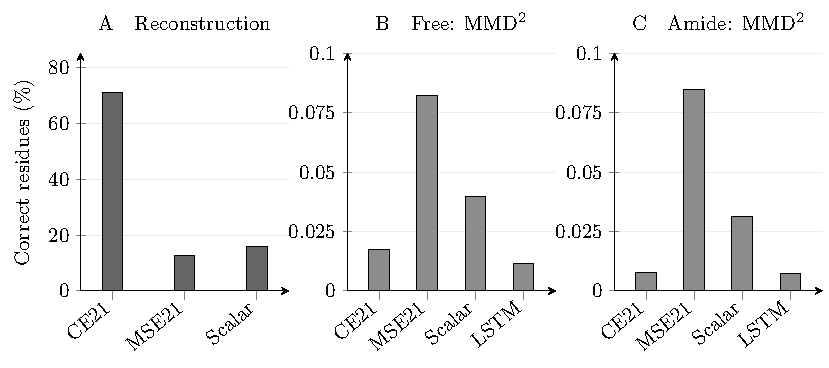
\includegraphics[width=\linewidth]{figures/reconstruction_generation.pdf}
\caption{CE21 improves both reconstruction and generation distances relative to MSE21, but the LSTM has smaller generation distances still. (A) Development residue reconstruction for the three VAE paths. (B,C) Development fixed-feature $\mmd$ for all four generators, with smaller values indicating closer feature means. Free and amidated conditions are shown separately. The autoregressive model has no reconstruction bar. All plotted values are descriptive results from one fitted seed; each generation group contains 16 requests. No uncertainty band is inferred from these draws.}\label{fig:results}
\end{figure}

The ordering is not uniform across all reported diagnostics. Scalar outputs have smaller absolute training-entropy discrepancies than CE21 for both residue and dipeptide entropy under both terminal conditions. CE21 also has fewer length-eligible outputs than scalar or LSTM. Thus neither ``all generation metrics improve'' nor ``all distributions worsen'' accurately describes the evidence. The descriptive recovery reconstruction screen passed its four checks; the generation screen failed eight of 18 checks. Those are decision-rule checks, not eight failed sequences, and they do not supersede the original interrupted protocol's status.

\subsection{Follow-up diagnostics did not establish an end-to-end repair}
The completed development sequence included additional frozen diagnostics, all preserved in the supplement. They are sequential investigations of already exposed data, not independent replications of the main comparison. Substituting training-posterior draws for diffusion draws did not lower development $\mmd$ in either terminal group. Independently permuting coordinates of those same sampled latents worsened this statistic, whereas a flow-prior route with residue-template information was mixed and had an unfair information advantage for model ranking.

A KL-warmup follow-up reduced the mean per-sequence posterior-mean reconstruction measure from 0.722796 to 0.657852 and the eight-draw measure from 0.661116 to 0.589099. A latent-conditioned autoregressive diagnostic subsequently showed substantial sequence information in the cached latent: its eight-draw sequence-level reconstruction score was 0.690802 with the matched latent and 0.097533 with a mismatched latent. Its generation gate nevertheless failed. These results separate information availability from successful sampling; they do not identify a unique causal bottleneck.

A direct-latent diffusion screen completed its fixed training but failed its prespecified mechanism screen. Independent checkpoint loading failed in the later audit; a restricted audit of saved sequences and scalar metrics passed. We therefore retain the negative observed screen while explicitly declining a full independent execution-reproduction claim. None of these follow-ups supplies a successful new generator or a justification for replacing the primary comparison with a selected favorable outcome.

\subsection{Activity evidence remains separate from sequence generation}
Exploratory MIC prediction on a separately acquired DBAASP development cache \citep{pirtskhalava2021} did not establish a reliable screening model. In native-unit source-group cross-prediction, a locally adapted convolutional architecture motivated by \citet{witten2019} had larger primary MAE than a training-mean predictor in both unit groups. A subsequent right-censoring likelihood comparison also failed to improve prediction on the observed point-valued validation subset. These were separate experiments with different cache versions and admission rules; neither selected nor validated the newly generated peptides. Their exact counts, methods and negative outcomes are reported in Supplementary Section S4.

The historical laboratory materials identify 27 peptides and a 27-by-four-strain MIC summary with 30 numeric entries and 78 entries marked ``N''. The meaning of N is unresolved. Under a transparent retrospective rule, six listed peptides have at least one numeric value strictly below 32~\ug, and seven have one below 128~\ug. These counts are not generation success rates. The source records disagree about the historical denominator and threshold, and a complete link from model checkpoint through selection to the 27 samples is unavailable. The full table and unresolved conflicts are preserved in Supplementary Section S5. No historical peptide is attributed to an H5 model.

\section{Discussion}
Within the fixed experiment, CE21 improves both reconstruction and the six sequence-distribution distances relative to the same-capacity MSE21 pipeline. The available recurrent generator nevertheless remains closer than CE21 on those distances. These are two different comparisons: the matched improvement is observed, whereas superiority over the separate autoregressive comparator is not. Because the LSTM has no corresponding reconstruction task, the results do not establish a reversal of reconstruction and generation rankings across the four models. This observation concerns the inspected operating point. It neither establishes the LSTM as a generally superior design method nor rejects posterior-parameter diffusion as a model class.

Several mechanisms could contribute to the remaining gap to the recurrent comparator. Reconstruction receives the input sequence and descriptors, whereas sampling receives a terminal condition. The learned posterior and the distribution sampled by diffusion can differ. The follow-up results show that cached latents contain decodable information, but do not isolate whether optimization, latent distribution, decoder behavior, loss scaling or limited data dominates the complete generation result. In particular, a fixed KL coefficient does not control the effective regularization strength when the reconstruction loss changes. Attribution to one component would require evidence not present here.

The results also illustrate why low-order distribution matching must retain complementary diagnostics. The selected distances omit biochemical activity, toxicity, stability and many higher-order sequence properties. Entropy and length eligibility can reverse part of the apparent ranking. A generation study should therefore report the full prespecified metric set, rejected and capped outputs, actual conditions, and the role of subsequent selection. Published AMP pipelines that include selection and laboratory assessment address a broader evidence chain than the sequence-only comparisons here \citep{szymczak2023}.

Relative to the broader comparison by \citet{beierle2026}, our distinctive evidence is the fixed implementation-level CE21 versus MSE21 comparison and its linked sampling result. Its additional scientific value and representativeness are not yet established; the fact that a comparator remains better is not itself a new general evaluation principle. Possible sharing of code, data, candidate peptides or assay materials with AMPGen remains to be clarified by the authors; overlapping authorship does not establish either duplication or independence.

The main limitations are substantial. The experiment uses one training seed, 16 requests per terminal group, and a repeatedly accessed development set. The recurrent baseline is executable but not demonstrated to be adequately optimized. Capacity and realized compute differ between model families. The CE recovery adds an interrupted-attempt history that must remain in the cost and execution record. The separate MIC cache is small, heterogeneous and already exposed; missing assay covariates and reporting selection preclude an unbiased activity-risk interpretation. The historical assay record lacks verified aggregation, replicate identities and model provenance.

An implementation-specific evaluation can be useful without introducing a new model, provided that its empirical scope and reproducibility justify the claims. The present record supports a bounded case study and an inspectable set of negative results. It does not yet support a representative benchmark, a general design recommendation, or a biologically validated application. The candidate is therefore complete for substantive review but remains blocked for submission by scientific scope and author-responsibility requirements, detailed in the accompanying decision sheet.

\section{Conclusion}
In this fixed AMP development experiment, categorical reconstruction improved reconstruction and low-order generation distances relative to the matched squared-error pipeline. It did not establish a better generator than the executed autoregressive comparator. Follow-up diagnostics and exploratory activity modeling did not close that gap. Historical peptide measurements remain historical evidence with unresolved semantics and provenance. These boundaries are part of the result and must remain visible in any subsequent manuscript.

\section*{Data and code availability}
The local review package contains the manuscript source, deterministic plotting source, source-bound summary data and supplementary tables. Configuration and source identifiers refer to the preserved AMP development artifacts. The inspected repository is \url{https://github.com/3DHumanRehab/AMP}; its public accessibility and a complete reusable release are not asserted. Model weights, complete input datasets and an archival public release are not included in this Overleaf package. A data-access, licensing and code-release arrangement acceptable to the journal remains outstanding. No external repository upload was performed for this candidate.

\section*{Use of generative AI tools}
The documented revision and H5 development used OpenAI Codex assistants for code inspection, implementation and debugging, experiment orchestration, statistical and provenance checks, literature and policy retrieval, substantive scientific drafting, LaTeX preparation and deterministic plotting code. Separate AI agents performed technical and scientific checks. The present manuscript was drafted with substantial AI assistance; assistance was not limited to language editing. No AI-generated illustration or newly simulated laboratory measurement is included. AI-agent checks are not human peer review. Exact historical model versions, the complete prior AI-use history and final human author verification remain unconfirmed. Named human authors must review and take responsibility for all content before submission; no such approval is represented as completed.

\section*{Funding}
The historical manuscript lists National Natural Science Foundation of China grants U22A2047 and 62371173. Their association with this work remains to be confirmed by the authors.
\section*{Author contributions and competing interests}
The author order, affiliations, corresponding-author details, individual contributions and competing-interest declarations require author confirmation. No contribution or absence of conflict has been inferred. No automated agent is listed as an author.

\bibliographystyle{plainnat}
\bibliography{references}
\end{document}
